\clearpage
\chapter{\textbf{Grundlagen}}\label{grundlagen}
%\addtocontents{toc}{\vspace{0.8cm}}

\section{Machine Learning}\label{unterkapitel}
\addtocontents{toc}{}%\vspace{0.8cm}}

Grundsätzlich beschreibt Machine Learning das Entwickeln mathematischer Modelle zur statistischen Auswertung
von Daten. Dabei wird dem Modell anhand von Daten zu einem bestimmten Sachverhalt beigebracht, in einem 
Datenset Schemata zu erkennen, womit sich eine Erwartung über die Umstände des Datensets treffen lässt.
Beispielsweise könnte ein solches Model aus einem Datenset mit der aktuellen Jahreszeit, Uhrzeit und 
Position der Sonne am Himmel trainiert werden, sodass es auch schließlich in einem anderen Datenset 
aus Jahreszeit und Position der Sonne Rückschlüsse auf die Uhrzeit treffen kann.\\
Als Vorbild für diesen ,,Lernvorgang'' dient das menschliche Gehirn, welches ebenfalls versucht zwischen 
bestimmten Input-Parametern wie z.B. der Form und Farbe eines Gegenstandes eine Beziehung herzustellen,
um das beobachtete Objekt in Zukunft schneller kategorisieren zu können.\\
Da eine Vielzahl von effektiven Machine Learning Algorithmen existiert, ist es essenziell, sich mit den
Stärken und Schwächen einzelner Herangehensweisen zu befassen.\newpage

Im Wesentlichen kann Machine Learning in zwei Unterkategorien unterteilt werden:
\begin{itemize}
    \item \textit{Supervised Learning} 
    \item \textit{Unsupervised Learning}
\end{itemize}
\textit{Supervised Learning} bedeutet zwischen bestimmten Feldern eines Datensets eine Beziehung
zu einem sog. Label herzustellen, welches als eine Art Ergebnis aus den Eingabewerten gesehen 
werden kann. Ein so traniertes Model kann dann neue, ihm vorher unbekannte Datensets, mit einem 
Label versehen - etwa wie in dem o.g. Beispiel wo Jahreszeit und Sonnenposition die Eingabewerte 
und die Uhrzeit das Label darstellen. Der Begriff ,,\textit{supervised}'' ergibt sich daraus, dass 
das Datenset, mit dem das Model traniert wird, diese Labels gegeben 
hat, sodass das Modell sich bei jedem Schritt des Lernvorgangs selbst korrigieren kann, falls 
eine Fehleinschätzung getroffen wurde.
Bei einer sog. ,,\textit{Klassifizierung}'' sind diese Labels fest vorgegeben, während sie in der 
,,\textit{Regression}'' kontinuierlicher Natur sind. Im Kontext dieser Arbeit wäre das Ergebnis einer 
Klassifizierung eine ,,1'' für Anwesenheit und eine ,,0'' für Abwesenheit, während das Ergebnis einer 
Regression eine Wahrscheinlichkeit auf Anwesenheit zwischen 0.0 und 1.0 darstellen würde.
\newline\newline
Beim ,,\textit{Unsupervised Learning}'' versucht das Modell ohne Referenz zu einem bestimmten 
Label, Zusammenhänge zwischen bestimmten Feldern des Datensets herzustellen. Solche Modelle 
arbeiten vorrangig mit ,,\textit{Clustering}'' und ,,\textit{Dimensionality Reduction}''.\\
,,\textit{Clustering}''-Algorithmen versuchen ein Datenset in kleinere Bereiche einzuteilen und
so aus den Feldern des Datensets bestimmte Abhängigkeiten abzuleiten.
\begin{figure}[h]
    \centering
    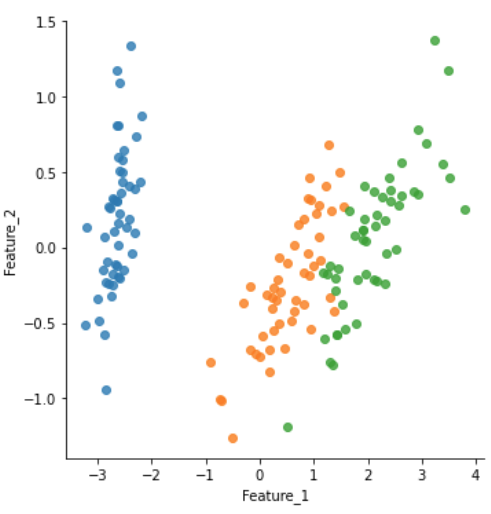
\includegraphics[width=8.0cm]{./pic/Clustering_Beispiel.png}
    \caption{Beispiel für Clustering}
    \label{fig:Clustering_Beispiel}
\end{figure}

Bei der ,,\textit{Dimensionality Reduction}'' versucht der Algorithmus das Datenset in einer 
Dimensionalität, also seiner Anzahl an Feldern, zu reduzieren. Es wird also die Frage gestellt, 
ob sich in einem bestehenden Datenset auch mit weniger Feldern Abhängigkeiten feststellen lassen. Dieser 
Schritt wird vorallem für Modelle benutzt, die sensibel gegenüber hoher Dimensionalitäten sind, 
sodass das Datenset vor dem Training in seiner Dimensionalität heruntergebrochen werden kann.

Im Rahmen des Projektes wurden hauptsächlich Klassifizierungs-Algorithmen genutzt, da ein Großteil der 
Datensets Labels zur Überprüfung hatte. Um einen Vergleich herzustellen werden später trotzdem noch 
einzelne Ergebnisse von Clustering und Dimensionality Reduction betrachtet. Im Folgenden sollen die genutzten 
Modelle erklärt werden.

\subsection{Random Forest Classifier}

Random Forests stellen eine Unterkategorien der ,,\textit{Decision Trees}'' dar. Decision Trees sind einfache
Anordnungen von bestimmten Fragen, die über das Datenset gestellt werden, um eine Klassifikation zu erreichen.

\begin{figure}[h]
    \centering
    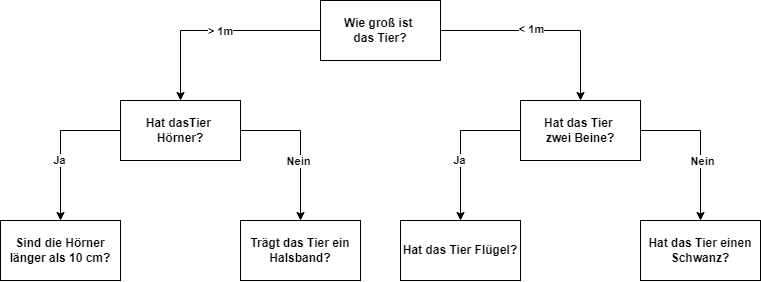
\includegraphics[width=10.0cm]{pic/DecisionTree.png}
    \caption{Beispiel eines Decision Trees}
    \label{fig:DT_Beispiel}
\end{figure}

Erstellt man ein ,,\textit{Ensemble}'' aus Decision Trees die Erwartungen über einen zufällig gewählten 
Teil des Datensets treffen können, entsteht ein Random Forest.
Der Random Forest Classifier versucht, eine Menge einfacher Schätzfunktionen über einen komplexeren 
Sachverhalt ,,abstimmen'' zu lassen. Während sich in einem einzelnen Entscheidungsbaum Fehleinschätzungen 
entwickeln können, sinkt die Chance auf eine solche Fehleinschätzung, je mehr unabhängige 
Entscheidungsbäume man befragt. 

\subsection{Support Vector Classifier}
Der Support Vector Classifier(SVC) versucht in einem Datenset anhand von bestimmten Cut-Off-Values klare Grenzen 
zwischen Werten zu finden, sodass man alle Messwerte ober- und unterhalb der Grenze eindeutig Klassifizieren 
kann.

\begin{figure}[h]
    \centering
    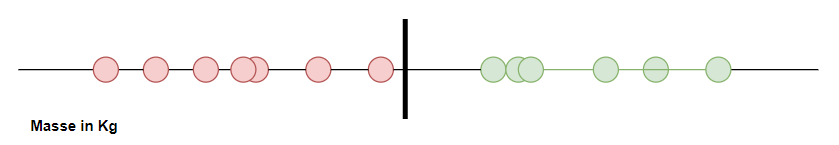
\includegraphics[width=10.0cm]{pic/SVC_1D.png}
    \caption{Beispiel eines Support Vector Classifiers}
    \label{fig:SVC_1D}
\end{figure}

In Abb. \ref{fig:SVC_1D} ist der SVC ein Punkt auf einer eindimensionalen Linie, auf der das Gewicht in Kg von z.B. 
Mäusen in ,,Unter-'' und ,,Übergewichtig'' unterteilt wird. Dieser Punkt ist Ergebnis aller Verhältnisse der einzelnen
Datenpunkte zueinander. Durch sog. ,,\textit{Kernel Funktionen}'' versucht der Algorithmus nun Beziehungen 
in höheren Dimensionen zu finden, wie z.B. $Masse^2$, $Masse^3$ usw. . Der SVC stellt dann in diesen Dimensionen 
eine Linie in einem zwei-dimensionalen oder eine Ebene in einem drei-dimensionalen Koordinatensystem dar.\\

\begin{figure}[h]
    \centering
    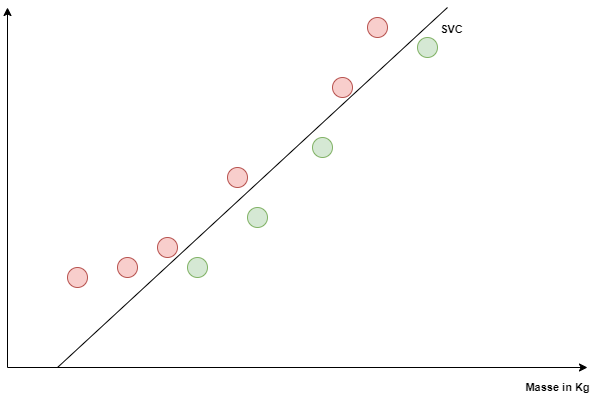
\includegraphics[width=10.0cm]{pic/SVC_2D.png}
    \caption{Beispiel eines Support Vector Classifiers in der zweiten Dimension}
    \label{fig:SVC_2D}
\end{figure}

Da der SVC die Verhältnisse aller Datenpunkte zueinander betrachtet, ist er sehr anfällig für Ausreißer in 
den Daten, was bei der Datenvorbereitung und der Auswertung beachtet werden muss.

\subsection{Gradient Boosting Classifier}
Der Gradien Boosting Classifier(GBC) versucht seine Erwartungen auf Grund von Abweichungen eines Labels vom 
Durchschnitt dieses Labels zu treffen. Erweitert man das Datenset im o.g. Beispiel um das Alter einer Maus, wird 
ein GBC als Ausgangswert den Durchschnitt aller Label-Werte, also dem Gewicht, berechnen. Danach werden die 
Abweichungen aller Label-Werte zu diesem Durchschnitt gebildet. Diese Abweichungen werden nun in Beziehung zu den 
anderen Spalten des Datensets gesetzt. Beispielsweise könnte man so davon ausgehen, dass ausgewachsene Mäuse von einem 
bestimmten Alter über dem Durchschnittsgewicht liegen. Genauso liegen besonders junge Mäuse wahrscheinlich immer
einen ähnlichen Wert unter dem Durchschnittsgewicht. So wurde zwischen dem Label \textit{Gewicht} und der Spalte 
\textit{Alter} eine Beziehung hergestellt. In weiteren Iterationen orientiert sich der GBC immer an der Abweichung 
zum Durchschnittswert des vorherigen Baumes. So werden die getroffenen Erwartungen über mehrere Iterationen immer 
präziser.\newpage

\subsection{Neuronale Netzwerke}
Die Funktionsweise eines Neuronalen Netzwerks ist direkt angelehnt an die Funktionsweise des menschlichen Gehirns.
Einzelne Knotenpunkten(Neuronen) werden mithilfe von Gewichteten Verbindungen verknüpft, sodass das Netzwerk versucht 
Eingabewerte bestimmten Ausgabewerten zuzuordnen. Diese Zuordnung der Ein- und Ausgabewerte im Input- und Output-Layer 
geschiet nicht direkt, sondern durch ein oder mehrere \textit{Hidden Layer}, dessen Neuronenzahl üblicherweise über 
der Anzahl Neuronen im Input Layer liegt. Die Anzahl der Neuronen im Output-Layer entspricht der Anzahl an Ergebnissen, 
die sich aus dem Input Ergeben können. Im Beispiel der Anwesenheitsanalyse entspräche das hier also zwei Neuronen für 
An- und Abwesenheit.

\begin{figure}[h]
    \centering
    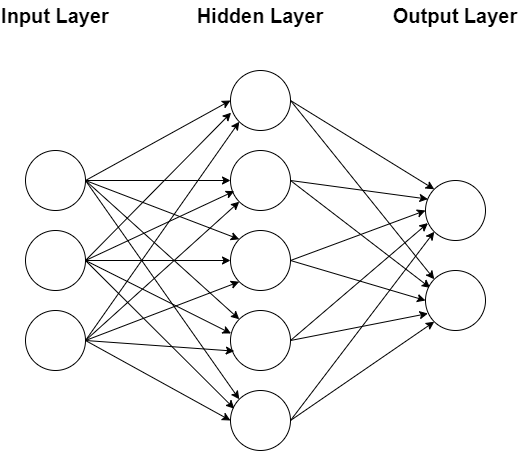
\includegraphics[width=10.0cm]{pic/NN.png}
    \caption{Beispiel eines neuronalen Netzwerks}
    \label{fig:NN}
\end{figure}

Liegt an einem Neuron eine Information an, wird diese als Eingabe einer Aktivierungsfunktion $\varphi$ genutzt, 
die mithilfe eines bestimmten Schwellwertes bestimmt, ob dieses Neuron aufgrund der Eingabe aktiviert wird. Über eine 
bestimmte Anzahl von Iterationen werden die Gewichtungen zwischen den einzelnen Neuronen stärker oder schwächer.


\subsection{Long Short Term Memory}
Das Long Short Term Memory (LSTM) ist eine Abwandlung herkömmlicher Neuronalen Netzwerke. Es handelt sich um ein
\textit{rekurrentes} Neurales Netzwerk, was bedeutet, dass jedes Neuron seine Ausgabewerte auch wieder als Eingabewerte
nutzt. Der Begriff \textit{Memory} rührt daher, dass durch diese Rückkopplung eine Art Gedächtnis entsteht, durch 
welches das Netzwerk bessere Rückschlüsse auf die Einordnung des aktuellen Input-Wertes ziehen kann.\\

\begin{figure}[h]
    \centering
    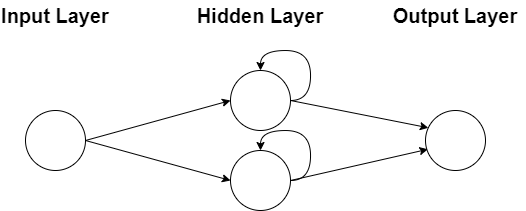
\includegraphics[width=10.0cm]{pic/RecurrentNN.png}
    \caption{Beispiel eines rekurrenten neuronalen Netzwerks}
    \label{fig:RecNN}
\end{figure}

Wird beispielsweise beim Satz ,,Das Auto ist Rot.'' das Wort ,,Das'' verarbeitet, kann das Netzwerk nun beim nächsten
Schritt eine zusätzliche Erwartung treffen, dass das nächste Wort wahrscheinlich nicht ebenfalls ,,Das'' sein wird.
Ein LSTM kann auf diese Weise eine Vielzahl von Zeitschritten zurückblicken und verlässt sich so nicht direkt auf 
einen gegebenen Input, sondern auf einen langen Verlauf von bereits verarbeiteten Input-Werten. 
LSTMs sind deshalb besonders interessant für Probleme bei denen Beziehungen zwischen kontinuierlichen 
Datenwerten gebildet werden müssen.\newpage

\section{CO2 als Anwesenheitsindikator}\label{CO2}

Der CO2-Gehalt der Raumluft ist als sehr guter Indikator für menschliche Präsenz anzusehen. Anders als andere 
Umweltindikatoren wie Temperatur oder Luftfeuchtigkeit hat der CO2-Gehalt die Eigenschaft, dass es in 
geschlossenen Räumen keine äußeren Einflussfaktoren für diesen Messwert gibt. In einem Büroraum kann der 
Mensch als alleinige Quelle für CO2 angesehen werden.\\
Der Anteil von CO2 in frischer Atemluft beträgt zwischen 350 und 450 ppm. Es gibt in Deutschland und auch Europa 
keine grundsätzlich festgelegten Grenzwerte für akzeptable Raumluft, vielmehr raten Gesundheitsämter 
verschiedener Länder Grenzwerte zwischen 1200 und 1500 ppm einzuhalten. Bei der Obergrenze von 1500 ppm 
entstehen beim Menschen erste Müdigkeitserscheinungen, weshalb dieser Wert in der Literatur als maximaler 
Richtwert für Innenräume gilt.

\begin{figure}[h]
    \centering
    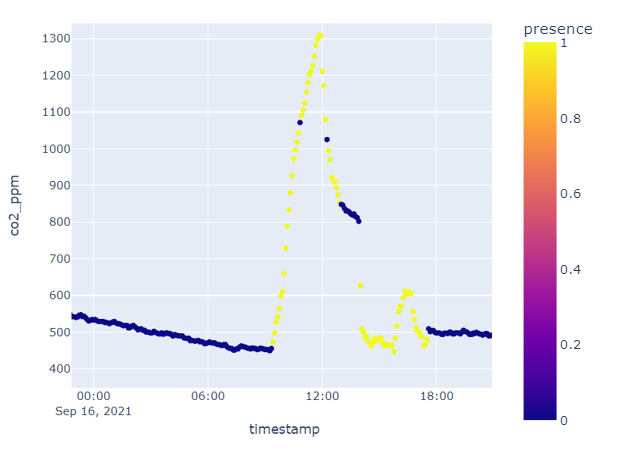
\includegraphics[width=0.7\textwidth]{pic/co2_singleDay.png}
    \caption{CO2 Gehalt der Raumluft über einen Tag}
    \label{fig:CO2_oneDay}
\end{figure}
 
Es ist zu erkennen, dass die CO2-Werte in einem normalen Büroraum innerhalb dieser empfohlenen Grenzen schwanken.
Mit einigen kleinen Pausen sind fast durchgehend Personen anwesend, die täglich etwa um 12:00 den Raum lüften.
Es ist auch klar zu erkennen, dass sich der CO2-Gehalt während Abwesenheit durch die passive Lüftung des Raumes  
(Tür-/Fensterspalten) langsam wieder gegen den Grundwert bewegt.

\section{Luftfeuchtigkeit und Temperatur}
Auch wenn Luftfeuchtigkeit und Temperatur Indikatoren für menschliche Präsenz in einem Raum sein können, 
unterliegen sie in ihrer Nützlichkeit dem CO2-Gehalt der Raumluft in einem wichtigen Faktor. 
Sie sich beide stark beeinlusst, von äußeren Umweltfaktoren wie dem aktuellen Wetter oder der Jahreszeit.
Beide Werte wurden zunächst in das Training aller Modelle miteinbezogen, es wird allerdings im Folgenden 
Kapitel gezeigt, dass diese beiden Werte zusammen mit dem CO2-Werte nicht von besonderem Nutzen sind und 
deshalb später nicht weiter genutzt werden.  

\section{Outlier Detection}
Wie bereits erwähnt, spielen Datenausreißer für die Ergebnisse mancher Algorithmen eine große Rolle. Überall 
wo z.B. aus einer Reihe von Datenwerten Durchschnittswerte berechnet werden, würden Ausreißer in den Daten das 
Ergebnis verfälschen und die Leistung des Algorithmus deutlich senken.
Um diese Ausreißer vor dem Training der Models zu beseitigen wurde das Verfahren des 
\textit{Interquartilabstands} (IQR nach der englischen Bezeichnung \textit{Interquartile Range}) gewählt.\\
Der IQR gibt die Intervallgröße an, die ein Wert vom Median einer Datenreihe abweichen darf. Bei einer 
der Größe nach sortierten Datenreihe $x = (x_0,x_1,...,x_n)$ bestimmt man die Mediane der unteren und oberen 
Hälfe des Datensets $Q_1$ und $Q_2$. Der IQR ergibt sich nun aus 

\begin{align}
    IQR = Q_2 - Q_1
\end{align}
Mit diesm Wert kann man nun die erlaubten Ober- und Untergrenzen 
des Datensets mit 
\begin{align}
    Limit_{upper} = Q_2 + 1.5 * IQR \\
    Limit_{lower} = Q_1 - 1.5 * IQR
\end{align} 
bestimmen. Alle Werte die außerhalb dieser Grenzen liegen, können als Ausreißer betrachtet werden.\\
Ausreißer zu entfernen, ist hier wichtig, da die Sensoren Messfehler erzeugen können, oder gelegentlich zur 
Demonstration von starken Veränderungen in der direkten Nähe des Sensors geatmet wurde und es so in vielen 
Datensets kurzfristige CO2-Werte gibt, die natürlich in geschlossenen Räumen nicht vorkommen.

\section{Sensordaten}
Wie bereits beschrieben, wurden die Sensordaten in mehreren Räumen der FH Aachen kontinuierlich 
gesammelt. Durch das Filtern nach der Beziehung des Raumes ergab sich folgende Datenstruktur als
Ausgangslage:\\

\begin{tabular}{|p{4.5cm}||p{3cm}|p{7cm}|}
    \hline
    \multicolumn{3}{|c|}{Sensordaten} \\
    \hline
    Name&Format &Beschreibung\\
    \hline
    timestamp&timestamp&Zeitpunkt der Messung\\
    co2\_ppm&integer&CO2-Wert\\
    temperature\_celsius&float&Temperatur in Grad Celsius\\
    relative\_humidity\_percent&float&Luftfeuchtigkeit\\
    presence&boolean&Aktivität des Bewegungssensors\\
    \hline
\end{tabular}     

\section{Datenbeschaffung und -Vorbereitung}
Die Daten wurden lokal auf einem der FH-Server in Form eines \textit{Hadoop Distributed File System} (HDFS) 
gespeichert. Mithilfe von Apache Drill konnten die Daten jederzeit mit einfachen SQL-Abfragen beschafft werden. 
Die Daten wurden so durch die gesamte Dauer des Projektes immer aktuell gehalten, damit alle Erkenntnisse 
immer auf der aktuellsten Datenlage basieren.
\\\\
Die Datenvorbereitung oder Pre-Processing ist eine der wichtigsten Schritte bei der Anwendung von Machine 
Learning. Durch sie kann man beim Training des Models durch Bearbeitung bestehender Spalten oder Hinzufügen 
von zusätzlichen Spalten im Datenset Schwerpunkte setzen, die es den Algorithmen beim Training zum einen 
erleichtern, ihre Erwartungen zu präzisieren, zum anderen aber auch die Leitung beim Verarbeiten bestimmter 
Spalten zu steigern.
\subsection{Gruppierung}
Die Sensordaten wurden alle sechs Sekunden erfasst. Da sich weder CO2-Gehalt noch Feuchtigkeits- oder 
Temperaturwerte der Raumluft so schnell nicht verändert, wurden die Daten direkt beim Drill per SQL zu 
zwei-Minuten-Intervallen zusammengefasst. Dabei werden über alle Spalten hinweg Durchschnittswerte gebildet, 
die dann nachher zu einem Datensatz zusammengefasst werden. 
Dies steigert die Leistung aller Algorithmen erheblich, da sich die Zahl der 
Datensätze um den Faktor 20 verringert. Da sich, wie oben erwähnt, der CO2-Gehalt der Raumluft in einem 
Intervall von zwei Minuten kaum merklich verändert, verringert sich die Genauigkeit des gesamten Datensetz 
dadurch nicht maßgeblich.
\subsection{Zyklische Codierung}
Zyklische Codierung wird immer dort verwendet, wo Daten sich in wiederholenden Schemata bewegen. Diese 
Schemata, wie z.B. die Zahlenumbrüche bei einer Uhrzeit, sind für Algorithmen nicht direkt ersichtlich und 
sind zudem für Computer nicht leicht zu verarbeiten. Durch eine Encodierung in 
Sinus- und Cosinus-Werte können diese Zusammenhänge vereinfacht werden.\\
Hierzu wurde der Timestamp zuerst in Sekunden übersetzt, sodass sich ein bestimmter Zeitpunkt eines Tages 
immer zwischen 0 und 86400 Sekunden bewegt.
Aus diesem Wert wurden dann zwei neue Datenspalten ,,\textit{hour\_sin}'' und ,,\textit{hour\_cos}'' 
in das Datenset eingefügt welche sich durch 

\begin{align}
    hour\_sin = sin(2 * \pi * x / x_{max}) \\ 
    hour\_cos = cos(2 * \pi * x / x_{max})
\end{align} 

ergeben. So kann jede Tageszeit einer eindeutigen Kombination aus Sinus- und Cosinus-Werten zwischen 
$0$ und $1$ zugeordnet werden.

\subsection{Deltas und Shift-Werte}
Desweiteren wurden von den Spalten ,,\textit{co2\_ppm}'', ,,\textit{temperature\_celsius}'' und \break 
,,\textit{relative\_humidity\_percent}'', die tatsächlich Rückschlüsse auf die Präsenz zulassen, \break 
zusätzliche Delta- und Shift-Spalten angelegt.\\\\
Ein Shift-Wert bedeutet lediglich, dass  in einer Zeile $x_n$ des Datensets 
zusätzlich, neben den aktuellen Werten, auch Werte von $k$ Zeilen zuvor, also $x_{n-k}$ stehen. So haben 
alle Algorithmen direkten Zugriff auf Vergangenheitswerte der ausgewählten Spalten.\\\\
Delta-Spalten stellen, dem Namen nach, Deltas zu vorherigen Werten dar:

\begin{align}
    \Delta x_k = x_n - x_{n-k}    
\end{align}

Die Erwartung ist hier, dass die Änderung der CO2-, Temperatur- und 
Luftfeuchtigkeitswerte ein wichtigerer Indikator sein könnte, als die tatsächlichen Werte. In einem schlecht 
klimatisierten Raum könnten Grundwerte von z.B. CO2 höher sein, als in anderen Räumen. Durch die hinzufügten 
Deltas werden diese Grundwerte ignoriert und Rückschlüsse auf die aktuelle Präsenz sind besser möglich.\\
Im Zuge der Projektarbeit wurden verschiedene Kombinationsmöglichkeiten von Delta- und Shiftwerten mit 
Zeitschritten zwischen zwei Minuten und einer Stunde mit Hinblick auf Verbesserungen der Model-Genauigkeiten 
getestet.

\subsection{Validierung}
\sloppy
Über das Projekt hinweg wurden verschiedene Validierungsmethoden verwendet. Grundsätzlich unterteilt man das 
Datenset in ein Trainings- und Testset mit einem Verhältnis von etwa 80-20. Das bedeutet, dass das Model mit
80 prozent der Daten trainiert wird, wobei die anderen 20 prozent zurückgehalten werden, um daraufhin das 
fertig trainierte Model daran zu testen. Aus dem Ergebnis dieses Tests ergibt sich ein Prozentwert, der die 
allgemeine Genauigkeit des Models repräsentiert, d.h. wie verlässlich das Model die An- und Abwesenheit des 
Testsets selbst berechnen kann, wenn man ihm den tatsächlichen Wert vorenthält.\\
Dieser Gesamtwert ist wiederrum der Durchschnitt der jeweiligen Genauigkeit beim errechnen von An- und 
Abwesenheit. In diesem Anwendungsfall ist es durchaus wichtig, beide Genauigkeiten einzeln zu betrachten, 
da ein Arbeitstag nur etwa ein Drittel eines tatsächlichen Tages darstellt. 
Das Datenset ist also mit einem Verhältnis von etwa 8/16 in Richtung der Abwesenheit unausgeglichen. Dies 
lässt die Erwartung zu, dass das trainierte Model wesentlich besser darin sein wird, Abwesenheit zu erkennen,
als Anwesenheit.\\
Hierzu wurde bei der Auswertung der Ergebnisse immer auch der \textit{Classification Report} hinzugezogen,
aus dem ersichtlich ist, wie genau das Model beide möglichen Labelwerte berrechnen konnte.\\\\
Desweiteren war es entscheidend zu erkennen, dass das Datenset über mehrere Monate hinweg nicht perfekt uniform 
ist, da es in bestimmten Monaten zu verhätlnismäßig vielen Urlaubstagen (z.B. Weihnachten/Silvester) und damit 
einer Häufung an Abwesenheits-Werten kommt.
Wenn die Daten nun im o.g. Verhältnis aufgeteilt werden und dann viele Daten des Testsets in solchen Monaten 
liegen, könnte es beim Ergebnis zu Verzerrungen kommen.\\
Hierfür wurde eine \textit{Kreuzvalidierung} (engl. Cross Validation) implementiert. Bei einer CV wird das 
Datenset immernoch im gleichen Verhältnis aufgeteilt, allerdings mehrmals, sodass die Trainings- und Testsets 
jedes mal aus jeweils anderen Daten bestehen.

\begin{figure}[h]
    \centering
    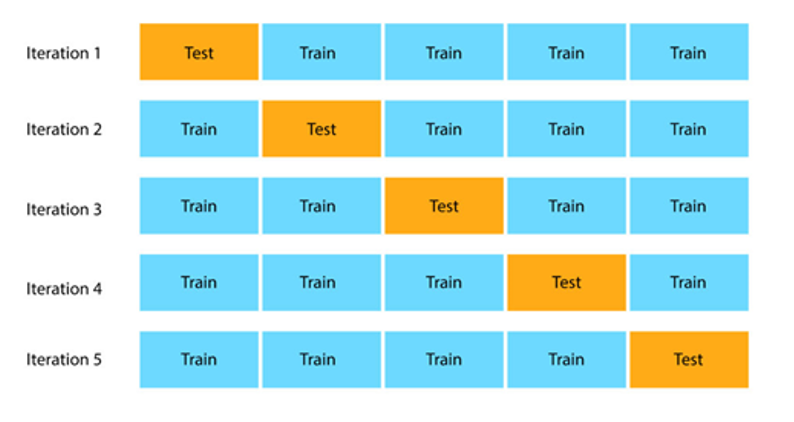
\includegraphics[width=0.7\textwidth]{pic/CV.png}
    \caption{Beispiel einer Kreuzvalidierung}
    \label{fig:CV}
\end{figure}

Errechnet man nun die Durchschnittsgenauigkeit aller Iterationen der CV, ergibt sich eine Gesamtgenauigkeit, 
die das Model besser repräsentiert, weil es an einer größeren Anzahl an verschiedenen Daten trainiert und 
getestet wurde.
\\\\
Da es für manche Räume keine Datensätze mit Labelwerten gab, musste die Validierung dieser Datensätze 
augenscheinlich erfolgen. Hierfür wurde in ein Datenset eine Labelspalte eingefügt, die dann vom trainierten
Model selbst gefüllt werden sollte. Das Ergebnis musste dann in einem Graphen gezeichnet und per Hand validiert 
werden. Da sich das Ergebnis der Berechnung in diesem Anwendungsfall, wie oben gezeigt, sehr übersichtlich als 
Graph darstellen lässt, war diese Methode der Validierung zwar nicht perfekt, lieferte aber trotzdem einen 
ausreichenden Eindruck über die Qualität des trainierten Models.
%% Zwei Abbildungen, die zusammen gehören

%\begin{figure}
%        \centering
%        \begin{minipage}[c]{0.45\textwidth}
%                \includegraphics[height=6.5cm]{pic/dateiname1.png}
%        \end{minipage}
%        \begin{minipage}[c]{0.45\textwidth}
%                \includegraphics[height=6.5cm]{pic/dateiname2.png}
%        \end{minipage}
%        \caption{Zwei Abbildungen}\label{fig:zwei_abb}
%\end{figure}
